% +==============================================================+
% |  Eksempel: Vandstandsstyring med PLC og Python               |
% |  Forfatter : aso                                             |
% |  Skole     : AAMS                                            |
% +==============================================================+

\documentclass[12pt, a4paper]{article}

% --- Kodning & sprog ----------------------------------------------------------
\usepackage[utf8]{inputenc}
\usepackage[T1]{fontenc}
\usepackage[danish]{babel}

% --- Layout -------------------------------------------------------------------
\usepackage{geometry}
\geometry{top=2.5cm, bottom=2.5cm, left=2.2cm, right=2.2cm, headheight=16pt}

% --- Typografi ----------------------------------------------------------------
\usepackage{lmodern}
\usepackage{microtype}
\usepackage{parskip}

% --- Grafik & farver ----------------------------------------------------------
\usepackage{graphicx}
\usepackage{xcolor}
\usepackage{tikz}
\usetikzlibrary{calc, arrows.meta, shapes.geometric, positioning, fit, backgrounds}

% --- Bokse & lister -----------------------------------------------------------
\usepackage[most]{tcolorbox}
\usepackage{enumitem}
\usepackage{booktabs}
\usepackage{multirow}
\usepackage{array}
\usepackage{tabularx}

% --- Kode-visning (listings) --------------------------------------------------
\usepackage{listings}

\definecolor{codebg}{HTML}{1E1E2E}
\definecolor{codetext}{HTML}{CDD6F4}
\definecolor{codecomment}{HTML}{6C7086}
\definecolor{codekeyword}{HTML}{CBA6F7}
\definecolor{codestring}{HTML}{A6E3A1}
\definecolor{codefunction}{HTML}{89DCEB}
\definecolor{codenumber}{HTML}{FAB387}

\lstdefinestyle{python}{
  language         = Python,
  backgroundcolor  = \color{codebg},
  basicstyle       = \ttfamily\small\color{codetext},
  keywordstyle     = \color{codekeyword}\bfseries,
  stringstyle      = \color{codestring},
  commentstyle     = \color{codecomment}\itshape,
  numberstyle      = \tiny\color{codenumber},
  numbers          = left,
  numbersep        = 24pt,
  breaklines       = true,
  tabsize          = 4,
  showstringspaces = false,
  frame            = none,
  xleftmargin      = 44pt,
  moredelim        = [is][\color{codefunction}]{|>}{<|},
  literate         =
    {æ}{{\ae}}1 {ø}{{\o}}1 {å}{{\aa}}1
    {Æ}{{\AE}}1 {Ø}{{\O}}1 {Å}{{\AA}}1,
}

% --- Hyperlinks ---------------------------------------------------------------
\usepackage{hyperref}
\hypersetup{
  colorlinks = true,
  linkcolor  = primaryblue,
  urlcolor   = accentblue,
}

% --- Header & footer ----------------------------------------------------------
\usepackage{fancyhdr}
\usepackage{titlesec}
\usepackage{fontawesome5}

% ==============================================================================
%  FARVEDEFINITIONER
% ==============================================================================
\definecolor{primaryblue}{HTML}{1A3A5C}
\definecolor{accentblue}{HTML}{2E86C1}
\definecolor{lightblue}{HTML}{D6EAF8}
\definecolor{darkgray}{HTML}{555555}
\definecolor{lightgray}{HTML}{F4F6F7}
\definecolor{successgreen}{HTML}{1E8449}
\definecolor{lightgreen}{HTML}{D5F5E3}
\definecolor{warnorange}{HTML}{E67E22}
\definecolor{lightyellow}{HTML}{FEF9E7}
\definecolor{siemensblue}{HTML}{009999}
\definecolor{passgreen}{HTML}{27AE60}
\definecolor{failred}{HTML}{C0392B}

% ==============================================================================
%  TCOLORBOX STILE
% ==============================================================================
\tcbset{
  infobox/.style={
    enhanced, colback=lightblue, colframe=accentblue,
    coltitle=white, fonttitle=\bfseries, arc=3pt, boxrule=1pt,
    title style={fill=accentblue},
  },
  tipbox/.style={
    enhanced, colback=lightgreen, colframe=successgreen,
    coltitle=white, fonttitle=\bfseries, arc=3pt, boxrule=1pt,
    title style={fill=successgreen},
  },
  warnbox/.style={
    enhanced, colback=lightyellow, colframe=warnorange,
    coltitle=white, fonttitle=\bfseries, arc=3pt, boxrule=1pt,
    title style={fill=warnorange},
  },
  defbox/.style={
    enhanced, colback=lightgray, colframe=primaryblue,
    coltitle=white, fonttitle=\bfseries, arc=3pt, boxrule=1pt,
    title style={fill=primaryblue},
  },
  codebox/.style={
    enhanced, colback=codebg, colframe=siemensblue,
    coltitle=white, fonttitle=\bfseries\small, arc=3pt, boxrule=1.5pt,
    title style={fill=siemensblue},
    top=2pt, bottom=2pt, left=0pt, right=0pt,
  },
}

% ==============================================================================
%  HEADER & FOOTER
% ==============================================================================
\pagestyle{fancy}
\fancyhf{}
\fancyhead[L]{\textcolor{darkgray}{\small\textit{Vandstandsstyring med PLC og Python}}}
\fancyhead[R]{\textcolor{siemensblue}{\small\faIndustry}\;\textcolor{darkgray}{\small\textit{AAMS | aso}}}
\fancyhead[C]{}
\renewcommand{\headrulewidth}{1pt}
\renewcommand{\headrule}{{\color{siemensblue}\hrule height 1pt width\headwidth}}
\fancyfoot[C]{\textcolor{darkgray}{\small\thepage}}
\fancyfoot[R]{\textcolor{darkgray}{\small\today}}

% ==============================================================================
%  SEKTIONSFORMATERING
% ==============================================================================
\titleformat{\section}
  {\color{primaryblue}\Large\bfseries}
  {\color{siemensblue}\thesection\hspace{6pt}\textcolor{siemensblue}{|}\hspace{6pt}}
  {0pt}{}[{\color{siemensblue}\titlerule[1pt]}]

\titleformat{\subsection}
  {\color{primaryblue}\large\bfseries}
  {\color{accentblue}\thesubsection\hspace{6pt}}
  {0pt}{}

\titleformat{\subsubsection}
  {\color{primaryblue}\normalsize\bfseries}
  {\color{darkgray}\thesubsubsection\hspace{6pt}}
  {0pt}{}

\titlespacing{\section}{0pt}{18pt}{8pt}
\titlespacing{\subsection}{0pt}{12pt}{4pt}
\titlespacing{\subsubsection}{0pt}{8pt}{3pt}

% ==============================================================================
%  TIKZ STILE
% ==============================================================================
\tikzset{
  block/.style={
    rectangle, rounded corners=3pt, draw=primaryblue, thick,
    fill=lightblue, text width=3.2cm, align=center,
    minimum height=1.1cm, font=\small\bfseries\color{primaryblue}
  },
  sensor/.style={
    rectangle, rounded corners=3pt, draw=successgreen, thick,
    fill=lightgreen, text width=2.5cm, align=center,
    minimum height=0.9cm, font=\small\bfseries\color{successgreen!70!black}
  },
  actuator/.style={
    rectangle, rounded corners=3pt, draw=warnorange, thick,
    fill=lightyellow, text width=2.5cm, align=center,
    minimum height=0.9cm, font=\small\bfseries\color{warnorange!80!black}
  },
  software/.style={
    rectangle, rounded corners=3pt, draw=siemensblue, thick,
    fill=siemensblue!10, text width=3.2cm, align=center,
    minimum height=1.1cm, font=\small\bfseries\color{siemensblue!80!black}
  },
  myarrow/.style={-{Stealth[length=6pt]}, thick, color=darkgray},
  dbarrow/.style={-{Stealth[length=6pt]}, thick, color=siemensblue, dashed},
  % State machine styles
  state/.style={
    circle, draw=primaryblue, very thick, fill=lightblue,
    minimum size=1.6cm, align=center, font=\small\bfseries\color{primaryblue}
  },
  statestart/.style={
    circle, draw=primaryblue, very thick, fill=siemensblue!30,
    minimum size=1.6cm, align=center, font=\small\bfseries\color{primaryblue}
  },
  statealarm/.style={
    circle, draw=failred, very thick, fill=red!10,
    minimum size=1.6cm, align=center, font=\small\bfseries\color{failred}
  },
  trans/.style={-{Stealth[length=6pt]}, very thick, color=accentblue},
  translabel/.style={font=\footnotesize\itshape, fill=white, inner sep=1.5pt, text=darkgray},
}

% ==============================================================================
%  DOKUMENT START
% ==============================================================================
\begin{document}

% -----------------------------------------------------------------------------
%  FORSIDE
% -----------------------------------------------------------------------------
\begin{titlepage}
\thispagestyle{empty}


\begin{tikzpicture}[remember picture, overlay]
  \fill[primaryblue]
    (current page.north west) rectangle
    ([yshift=-4.5cm] current page.north east);
  \fill[siemensblue]
    ([yshift=-4.5cm] current page.north west) rectangle
    ([yshift=-5.0cm] current page.north east);
  \fill[accentblue]
    ([yshift=-5.0cm] current page.north west) rectangle
    ([yshift=-5.15cm] current page.north east);

  \node[anchor=east, xshift=-1.5cm, yshift=-2.3cm]
    at (current page.north east)
    {\textcolor{white!20!primaryblue}{\fontsize{90}{90}\selectfont\faIndustry}};

  \node[anchor=north west, xshift=2cm, yshift=-0.7cm]
    at (current page.north west)
    {\textcolor{white!70!primaryblue}\large\bfseries AAMS --- Automationsteknolog};

  \node[anchor=north west, xshift=2cm, yshift=-1.3cm]
    at (current page.north west)
    {\textcolor{white!60!primaryblue}\normalsize Teknologi og Projektudvikling $\cdot$ 2.\ Semester};

  \node[anchor=north west, xshift=2cm, yshift=-2.2cm]
    at (current page.north west)
    {\textcolor{white}{\fontsize{22}{28}\selectfont\bfseries Eksempel: Vandstandsstyring}};

  \node[anchor=north west, xshift=2.1cm, yshift=-3.2cm]
    at (current page.north west)
    {\textcolor{white!80!siemensblue}\large\itshape
     PLC + \texttt{snap7} + CSV-logging --- et fuldt gennemgange\-t eksempel};

  \node[anchor=north west, xshift=2.1cm, yshift=-3.85cm]
    at (current page.north west)
    {\textcolor{white!60!accentblue}\normalsize
     Kravspec.\ $\rightarrow$ Design $\rightarrow$ Kodning $\rightarrow$ Test};

  \fill[lightgray]
    ([yshift=3.5cm] current page.south west) rectangle
    ([yshift=2.0cm] current page.south east);
  \fill[accentblue]
    ([yshift=3.5cm] current page.south west) rectangle
    ([yshift=3.35cm] current page.south east);

  \node[anchor=west, xshift=2cm, yshift=2.8cm]
    at (current page.south west)
    {\textcolor{primaryblue}{\faUserCircle\quad\textbf{Forfatter:} aso
     \quad\textcolor{darkgray}{|}\quad
     \faCalendar\quad\textbf{Dato:} \today
     \quad\textcolor{darkgray}{|}\quad
     \faUniversity\quad\textbf{Skole:} AAMS}};
\end{tikzpicture}

\vspace*{5.5cm}

\begin{center}
\begin{tcolorbox}[
  enhanced, width=13cm, colback=lightgray, colframe=primaryblue,
  arc=5pt, boxrule=1.5pt,
  title={\faInfoCircle\quad Formål med dette dokument},
  coltitle=white, fonttitle=\bfseries, title style={fill=primaryblue},
]
Dette dokument viser, hvordan V-modellens processer bruges i praksis.
Vi følger et fuldt eksempel fra kravspecifikation til accepttest for et
\textbf{pumpeanlæg med vandstandsmåling}.

\vspace{6pt}
\begin{itemize}[leftmargin=1.2em, itemsep=4pt]
  \item[\textcolor{siemensblue}{\faCheckCircle}]
    Skriv en kravspecifikation med K0x-krav og acceptkriterier
  \item[\textcolor{siemensblue}{\faCheckCircle}]
    Tegn blokdiagram og state machine
  \item[\textcolor{siemensblue}{\faCheckCircle}]
    Implementer Python-kode med \texttt{snap7}, docstrings og CSV-logging
  \item[\textcolor{siemensblue}{\faCheckCircle}]
    Gennemfør og dokumentér FAT og accepttest
\end{itemize}
\end{tcolorbox}
\end{center}

\end{titlepage}

% -----------------------------------------------------------------------------
%  INDHOLDSFORTEGNELSE
% -----------------------------------------------------------------------------
\newpage
\thispagestyle{fancy}
\tableofcontents
\newpage

% ==============================================================================
\section{Systembeskrivelse}
% ==============================================================================

\subsection{Formål}

Systemet skal holde vandstanden i en tank inden for et ønsket interval ved at
styre en pumpe via en Siemens S7{-}1200 PLC\@.
En Python-applikation på en PC forbinder til PLC'en via Snap7 over Ethernet,
læser vandstand og pumpestatus hvert sekund og logger data til en CSV-fil.

\subsection{Projektomfang}

\begin{tcolorbox}[infobox, title={\faInfoCircle\quad Hvad er med og hvad er ikke med}]
\textbf{Er med:}
\begin{itemize}[leftmargin=1.2em, itemsep=2pt]
  \item Automatisk start/stop af pumpe baseret på vandstand
  \item Alarmhåndtering ved for højt niveau eller kommunikationsfejl
  \item Kontinuerlig datalogning til CSV med tidsstempel
\end{itemize}
\vspace{4pt}
\textbf{Er ikke med:}
\begin{itemize}[leftmargin=1.2em, itemsep=2pt]
  \item HMI-visualisering (kan tilføjes i et efterfølgende trin)
  \item Fjernalarmering (SMS, e-mail)
\end{itemize}
\end{tcolorbox}

\subsection{Komponenter}

\begin{center}
\begin{tabular}{llll}
\toprule
\textbf{Komponent} & \textbf{Type} & \textbf{Tilslutning} & \textbf{Bemærkning} \\
\midrule
PLC                & Siemens S7{-}1200     & ---               & Styreenhed \\
Niveau-sensor      & Digital, \textit{NC}  & I0.0              & Aktivt når niveau < 20\,\% \\
Overflow-switch    & Digital, \textit{NC}  & I0.1              & Aktivt ved overløb \\
Pumpe              & Digital output        & Q0.0              & 24\,V DC relæ \\
PC (Python)        & Ethernet              & DB1               & Snap7-klient \\
\bottomrule
\end{tabular}
\end{center}

% ==============================================================================
\section{Kravspecifikation}
% ==============================================================================

\subsection{Funktionelle krav}

\begin{tcolorbox}[infobox, title={\faInfoCircle\quad Læs inden du bruger kravene}]
Hvert krav har et unikt ID (K0x), en beskrivelse og et \textbf{acceptkriterie}.
Her betyder acceptkriteriet den målbare observation, du bruger til at
\textbf{verificere} kravet i FAT eller systemtest.

\vspace{4pt}
Det er \textbf{ikke} det samme som den afsluttende accepttest i V-modellen.
Accepttesten (UAT) ligger til sidst og bruges til at \textbf{validere}, at den
samlede løsning giver mening for brugeren i praksis.
\end{tcolorbox}

\vspace{0.3cm}
\begin{tabularx}{\textwidth}{lXX}
\toprule
\textbf{ID} & \textbf{Krav} & \textbf{Acceptkriterie} \\
\midrule
K01 & Pumpen skal starte automatisk, når vandstanden falder til under 20\,\%. &
  Python setter DB1.DBX0 bit\,0 = 1, og Q0.0 = \texttt{TRUE} bekræftes i PLC\@. \\[6pt]

K02 & Pumpen skal stoppe automatisk, når vandstanden når 80\,\%. &
  Python setter DB1.DBX0 bit\,1 = 1, og Q0.0 = \texttt{FALSE} bekræftes. \\[6pt]

K03 & Systemet skal gå i ALARM-tilstand ved overflow (I0.1 = 1). &
  DB1.DBX6 sættes til 1 af PLC'en, Python skifter til ALARM-state og stopper pumpem. \\[6pt]

K04 & Systemet skal logge vandstand, pumpestatus og alarmkode til CSV hvert sekund. &
  CSV-fil indeholder rækker med maks.\ 1\,s mellemrum og korrekte kolonner. \\[6pt]

K05 & Systemet skal håndtere Snap7-fejl uden at gå ned --- fejl skal logges og forbindelsen genoprettes. &
  Ved netværksafbrud prøver scriptet igen hvert 5\,s og logger fejlen til CSV\@. \\
\bottomrule
\end{tabularx}

\vspace{0.4cm}
\subsection{Ikke-funktionelle krav}

\begin{tabularx}{\textwidth}{lX}
\toprule
\textbf{ID} & \textbf{Krav} \\
\midrule
NK01 & Opdateringsinterval må ikke overstige 1{,}5\,s under normal drift. \\[4pt]
NK02 & CSV-filnavn dannes automatisk ud fra opstartstidspunkt (format: \texttt{YYYY-MM-DD\_HHMMSS.csv}). \\[4pt]
NK03 & Python-scriptet skal have kommentarer der forklarer hver logisk del. \\
\bottomrule
\end{tabularx}

% ==============================================================================
\section{Systemdesign}
% ==============================================================================

\subsection{Blokdiagram}

Blokdiagrammet viser systemets hoveddele og dataflow.
Sensorer og aktuatorer er tilkoblet PLC'en.
PC'en kommunikerer med PLC'en via Snap7 over Ethernet og læser/skriver
data i DB1.

\vspace{0.5cm}
\begin{center}
\scalebox{0.82}{
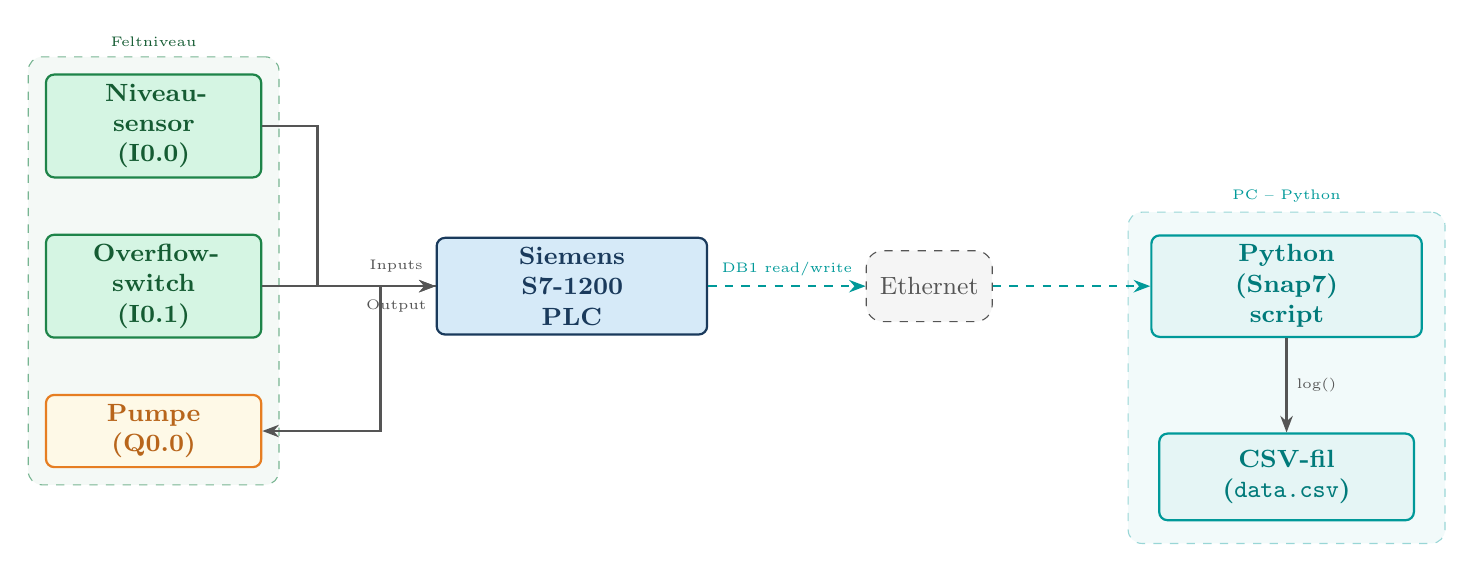
\begin{tikzpicture}[node distance=1.2cm and 2.4cm]

  % --- Hardware-lag ---
  \node[sensor] (niv)  {Niveau-\\sensor\\(I0.0)};
  \node[sensor, below=0.7cm of niv] (ovf) {Overflow-\\switch\\(I0.1)};
  \node[actuator, below=0.7cm of ovf] (pump) {Pumpe\\(Q0.0)};

  % --- PLC ---
  \node[block, right=2.2cm of ovf] (plc) {Siemens\\S7-1200\\PLC};

  % --- Ethernet-sky ---
  \node[draw=darkgray, dashed, rounded corners=6pt, fill=gray!8,
        minimum width=1.6cm, minimum height=0.9cm,
        right=2.0cm of plc, yshift=0.0cm, font=\small\color{darkgray}]
        (eth) {Ethernet};

  % --- PC / Python ---
  \node[software, right=2.0cm of eth] (py) {Python\\(Snap7)\\script};

  % --- CSV ---
  \node[software, below=1.2cm of py, text width=3.0cm] (csv)
        {CSV-fil\\(\texttt{data.csv})};

  % --- Forbindelser sensorer -> PLC ---
  \draw[myarrow] (niv.east)  -- ++(0.7,0) |- (plc.west);
  \draw[myarrow] (ovf.east)  -- (plc.west);
  \draw[myarrow] (plc.west)  -- ++(-0.7,0) |- (pump.east);

  % --- Label på PLC input/output ---
  \node[font=\tiny\color{darkgray}, above=0.05cm of plc.west, xshift=-0.5cm]
    {Inputs};
  \node[font=\tiny\color{darkgray}, below=0.05cm of plc.west, xshift=-0.5cm]
    {Output};

  % --- PLC <-> Ethernet <-> Python ---
  \draw[dbarrow] (plc.east) -- node[above, font=\tiny\color{siemensblue}]
    {DB1 read/write} (eth.west);
  \draw[dbarrow] (eth.east) -- (py.west);

  % --- Python -> CSV ---
  \draw[myarrow] (py.south) -- node[right, font=\tiny\color{darkgray}]
    {log()} (csv.north);

  % --- Grupperingsrammer ---
  \begin{scope}[on background layer]
    \node[draw=successgreen!60, dashed, rounded corners=5pt,
          fit=(niv)(ovf)(pump), inner sep=6pt,
          fill=successgreen!5, label={[font=\tiny\color{successgreen!70!black}]above:
          Feltniveau}] {};
    \node[draw=siemensblue!40, dashed, rounded corners=5pt,
          fit=(py)(csv), inner sep=8pt,
          fill=siemensblue!5, label={[font=\tiny\color{siemensblue}]above:
          PC -- Python}] {};
  \end{scope}

\end{tikzpicture}
}
\end{center}
\vspace{0.3cm}

\subsection{DB1 --- datablok-struktur}\label{sec:db1}

PLC'en eksponerer en datablok (\textbf{DB1}) som Python-scriptet læser og skriver til.

\begin{center}
\begin{tabular}{cclll}
\toprule
\textbf{Offset} & \textbf{Snap7 addr.} & \textbf{Type} & \textbf{Navn} & \textbf{Beskrivelse} \\
\midrule
DBX0   & byte 0, bit 0 & BOOL & PumpStart     & Python skriver 1 for at starte pumpe \\
DBX0   & byte 0, bit 1 & BOOL & PumpStop      & Python skriver 1 for at stoppe pumpe \\
DBX1   & byte 1, bit 0 & BOOL & PumpRunning   & PLC skriver 1 når pumpe kører \\
DBX1   & byte 1, bit 1 & BOOL & PumpFault     & PLC skriver 1 ved motorværnsfejl \\
DBX2   & byte 2--5     & REAL & WaterLevel    & Vandstand i \% (0.0--100.0) \\
DBX6   & byte 6--7     & INT  & AlarmCode     & 0=OK, 1=Overflow, 2=CommFault \\
\bottomrule
\end{tabular}
\end{center}

% ==============================================================================
\section{Moduldesign}
% ==============================================================================

\subsection{State machine --- Python-script}

State machinen beskriver de mulige tilstande i Python-scriptet og betingelserne
for at skifte imellem dem.

\begin{center}
\begin{tikzpicture}[node distance=3.2cm]

  % --- Nodes ---
  \node[statestart] (idle)  {IDLE};
  \node[state, right=of idle]  (fill)  {FILL};
  \node[statealarm, below=of fill] (alarm) {ALARM};
  \node[state, left=of alarm]  (reset) {RESET};

  % --- Start-pil ---
  \draw[trans] ([yshift=1.2cm]idle.north) -- node[translabel, right]{Start} (idle.north);

  % --- IDLE -> FILL ---
  \draw[trans] (idle.east) -- node[translabel, above]
    {level < 20\,\%} (fill.west);

  % --- FILL -> IDLE ---
  \draw[trans] (fill.west) to[bend left=20]
    node[translabel, below] {level $\geq$ 80\,\%} (idle.east);

  % --- FILL -> ALARM ---
  \draw[trans] (fill.south) -- node[translabel, right]
    {AlarmCode $\neq$ 0} (alarm.north);

  % --- IDLE -> ALARM ---
  \draw[trans] (idle.south) to[bend right=15]
    node[translabel, left] {AlarmCode $\neq$ 0} (alarm.west);

  % --- ALARM -> RESET ---
  \draw[trans] (alarm.west) -- node[translabel, above]
    {Pumpe stoppet} (reset.east);

  % --- RESET -> IDLE ---
  \draw[trans] (reset.north) to[bend right=15]
    node[translabel, right] {AlarmCode = 0} (idle.south);

  % Farveforklaring
  \node[below=0.5cm of alarm, font=\small\color{darkgray}]
    {\faExclamationTriangle\; ALARM-state: pumpe stoppes øjeblikkeligt};

\end{tikzpicture}
\end{center}

\subsection{Flowchart --- Python-hoved\-løkke}

\begin{center}
\begin{tikzpicture}[
  every node/.style={font=\small},
  process/.style={rectangle, rounded corners=2pt, draw=primaryblue, fill=lightblue,
                  text width=5cm, align=center, minimum height=0.8cm},
  decision/.style={diamond, aspect=2.8, draw=accentblue, fill=accentblue!15,
                   text width=3.6cm, align=center, inner sep=1pt},
  term/.style={rectangle, rounded corners=8pt, draw=primaryblue, fill=primaryblue!80,
               text=white, text width=4cm, align=center, minimum height=0.8cm},
  fl/.style={-{Stealth[length=5pt]}, thick, color=darkgray},
  node distance=0.55cm,
]

  \node[term] (start) {START};
  \node[process, below=of start] (conn) {Forbind til PLC\\(\texttt{client.connect()})};
  \node[process, below=of conn]  (open) {Åbn CSV-fil\\(\texttt{open(..., 'w')})};
  \node[process, below=of open]  (loop) {Update input\\(\texttt{db\_read()})};
  \node[process, below=of loop]  (parse){Program / logik\\(state machine)};
  \node[decision, below=0.4cm of parse] (statedec)
    {Start, stop\\eller alarm?};
  \node[process, below=0.5cm of statedec] (log)
    {Update output + log\\(\texttt{db\_write()} + \texttt{writer.writerow()})};
  \node[process, below=of log]   (sleep){Vent 1 sekund\\(\texttt{time.sleep(1)})};
  \node[decision, below=0.4cm of sleep] (intr)
    {Keyboard\\Interrupt?};
  \node[term, below=0.5cm of intr] (stop)
    {Luk CSV og\\afbryd PLC};

  % --- Pile ---
  \draw[fl] (start) -- (conn);
  \draw[fl] (conn)  -- (open);
  \draw[fl] (open)  -- (loop);
  \draw[fl] (loop)  -- (parse);
  \draw[fl] (parse) -- (statedec);
  \draw[fl] (statedec) -- (log);
  \draw[fl] (log)   -- (sleep);
  \draw[fl] (sleep) -- (intr);
  \draw[fl] (intr)  -- node[right]{Ja} (stop);

  % Tilbageloop
  \draw[fl] (intr.east) -- ++(1.3,0)
    node[above, font=\footnotesize\color{darkgray}]{Nej}
    -- ++(0,7.5)
    |- (loop.east);

  % Fejlhåndtering note
  \node[draw=warnorange, rounded corners=2pt, fill=lightyellow,
        right=0.5cm of conn, text width=3.5cm, align=left,
        inner sep=5pt, font=\footnotesize]
    (snap7err)
    {\textcolor{warnorange}{\faExclamationTriangle\;\textbf{Fejl:}}\\
     \texttt{try/except} fanget $\rightarrow$\\
     log fejl, vent 5\,s, forsøg igen};
  \draw[-{Stealth[length=4pt]}, dashed, color=warnorange]
    (conn.east) -- (snap7err.west);

\end{tikzpicture}
\end{center}
\clearpage

% ==============================================================================
\section{Kodning}
% ==============================================================================

\begin{tcolorbox}[infobox, title={\faInfoCircle\quad Inden du læser koden}]
Læg mærke til:
\begin{itemize}[leftmargin=1.2em, itemsep=2pt]
  \item Koden er skrevet \textbf{uden funktioner} --- alt kører i én sekvens fra toppen
  \item Hver cyklus følger et simpelt scan-princip: update input $\rightarrow$ program/logik $\rightarrow$ update output og log
  \item CSV-filnavnet dannes automatisk af opstartstidspunktet (NK02)
  \item State machinen ligger i program/logik-delen som en \texttt{if/elif}-blok
  \item Snap7-fejl fanges med \texttt{try/except} --- scriptet stopper ikke (K05)
\end{itemize}
\end{tcolorbox}

\vspace{0.3cm}

% --- Del 1: imports og indstillinger ----------------------------------------
\begin{tcolorbox}[codebox,
  title={\faPython\quad \texttt{vandstand.py} \textnormal{\textcolor{white!60!siemensblue}{\small --- del 1/4: imports og indstillinger}}}]
\begin{lstlisting}[style=python]
import snap7
import csv
import time
from datetime import datetime
from snap7.util import get_real, get_int, get_bool, set_bool

# Indstillinger
PLC_IP   = "192.168.0.1"
RACK     = 0          # Rack 0 for S7-1200
SLOT     = 1          # Slot 1 for S7-1200
DB_NR    = 1          # Datablok DB1
INTERVAL = 1.0        # Sekunder mellem hvert maal
RETRY_DELAY = 5.0     # Sekunder mellem genforsoeg ved fejl

# CSV-filnavn dannes automatisk (opfylder NK02)
filnavn = datetime.now().strftime("%Y-%m-%d_%H%M%S") + ".csv"
\end{lstlisting}
\end{tcolorbox}

\vspace{0.3cm}

% --- Del 2: forbind + aaben CSV ----------------------------------------------
\begin{tcolorbox}[codebox,
  title={\faPython\quad \texttt{vandstand.py} \textnormal{\textcolor{white!60!siemensblue}{\small --- del 2/4: forbind og aaben CSV}}}]
\begin{lstlisting}[style=python, firstnumber=18]
# Forbind til PLC
client = snap7.client.Client()
while not client.get_connected():
    try:
        client.connect(PLC_IP, RACK, SLOT)
        if client.get_connected():
            print("Forbundet til PLC.")
    except Exception as e:
        print("Fejl ved forbindelse:", e)
        time.sleep(RETRY_DELAY)

# Aaben CSV-fil og skriv kolonneoverskrifter
with open(filnavn, "w", newline="", encoding="utf-8") as csv_fil:
    writer = csv.writer(csv_fil)
    writer.writerow(["timestamp", "state", "vandstand_pct",
                     "pumpe_koerer", "alarmkode"])

    # Start-tilstand for state machine
    state = "IDLE"
\end{lstlisting}
\end{tcolorbox}

\vspace{0.3cm}

% --- Del 3: while-loekke og state machine ------------------------------------
\begin{tcolorbox}[codebox,
  title={\faPython\quad \texttt{vandstand.py} \textnormal{\textcolor{white!60!siemensblue}{\small --- del 3/4: update input og program/logik}}}]
\begin{lstlisting}[style=python, firstnumber=38]
try:
  while True:
    try:
      # 1. Update input: laes seneste data fra PLC
      data = client.db_read(DB_NR, 0, 8)

      # Udtaek vaerdier fra bytearray
      vandstand = get_real(data, 2)     # DBX2: vandstand 0-100 %
      pumpe_paa = get_bool(data, 1, 0)  # DBX1 bit0: pumpe koerer
      alarmkode = get_int(data, 6)      # DBX6: 0=OK, 1=Overflow

      # 2. Program/logik: beregn naeste state og kommandoer
      start_cmd = False
      stop_cmd = False

      if state == "IDLE":
        if alarmkode != 0:
          state = "ALARM"
        elif vandstand < 20.0:
          start_cmd = True
          state = "FILL"

      elif state == "FILL":
        if alarmkode != 0:
          state = "ALARM"
        elif vandstand >= 80.0:
          stop_cmd = True
          state = "IDLE"

      elif state == "ALARM":
        stop_cmd = True
        state = "RESET"

      elif state == "RESET":
        if alarmkode == 0:
          state = "IDLE"
\end{lstlisting}
\end{tcolorbox}

\vspace{0.3cm}

% --- Del 4: log + afslutning -------------------------------------------------
\begin{tcolorbox}[codebox,
  title={\faPython\quad \texttt{vandstand.py} \textnormal{\textcolor{white!60!siemensblue}{\small --- del 4/4: update output, log og fejlhaandtering}}}]
\begin{lstlisting}[style=python, firstnumber=77]
      # 3. Update output og log
      cmd = client.db_read(DB_NR, 0, 1)
      set_bool(cmd, 0, 0, start_cmd)
      set_bool(cmd, 0, 1, stop_cmd)
      client.db_write(DB_NR, 0, cmd)

      ts = datetime.now().strftime("%Y-%m-%d %H:%M:%S")
      writer.writerow([ts, state, f"{vandstand:.1f}",
               int(pumpe_paa), alarmkode])
      csv_fil.flush()

      print(f"{ts}  {state}  Vandstand: {vandstand:.1f}%")

      # 4. Vent foer naeste cyklus
      time.sleep(INTERVAL)

    except Exception as e:
      print("Snap7-fejl:", e)

      ts = datetime.now().strftime("%Y-%m-%d %H:%M:%S")
      writer.writerow([ts, "COMM_ERROR", "", "", 2])
      csv_fil.flush()

      client.disconnect()
      time.sleep(RETRY_DELAY)

      while not client.get_connected():
        try:
          client.connect(PLC_IP, RACK, SLOT)
          if client.get_connected():
            print("Forbundet til PLC igen.")
        except Exception as reconnect_error:
          print("Fejl ved genforbindelse:", reconnect_error)
          time.sleep(RETRY_DELAY)

except KeyboardInterrupt:
  print("Stoppet af bruger (Ctrl+C)")

finally:
  if client.get_connected():
    client.disconnect()
  print(f"Data gemt i: {filnavn}")
\end{lstlisting}
\end{tcolorbox}
\clearpage

% ==============================================================================
\section{Testdokumentation}
% ==============================================================================

\subsection{Factory Acceptance Test (FAT)}\label{sec:fat}

FAT udføres på labben, inden systemet evt.\ flyttes til driftsmiljøet.
Her \textbf{verificeres} kravene ét for ét mod deres acceptkriterier.

\begin{tcolorbox}[warnbox, title={\faExclamationTriangle\quad Inden testen}]
Sørg for at PLC-programmet er indlæst og kørende, og at DB1 er oprettet med
den korrekte struktur (se afsnit~\ref{sec:db1}).
Kontrollér at netværksforbindelsen til PLC er tilgængelig (\texttt{ping 192.168.0.1}).
\end{tcolorbox}

\vspace{0.4cm}

\begin{tabularx}{\textwidth}{p{1cm} p{2.6cm} p{3.8cm} p{3.8cm} p{1.5cm}}
\toprule
\textbf{Krav} & \textbf{Testbetingelse} & \textbf{Forventet resultat} & \textbf{Faktisk resultat} & \textbf{Status} \\
\midrule
K01 &
  Sæt WaterLevel (DBX2) til 15{,}0 i PLC-watch &
  Script skifter til FILL, sender StartPump, Q0.0 går HIGH &
  \textit{(udfyldes)} &
  \textcolor{passgreen}{\textbf{P}} \;/\; \textcolor{failred}{\textbf{F}} \\[6pt]

K02 &
  Kør script med level stigende --- sæt DBX2 til 82{,}0 &
  Script skifter til IDLE, sender StopPump, Q0.0 går LOW &
  \textit{(udfyldes)} &
  \textcolor{passgreen}{\textbf{P}} \;/\; \textcolor{failred}{\textbf{F}} \\[6pt]

K03 &
  Sæt DBX6 til 1 (overflow) mens system er i FILL &
  Script skifter til ALARM, stopper pumpen, logger ALARM &
  \textit{(udfyldes)} &
  \textcolor{passgreen}{\textbf{P}} \;/\; \textcolor{failred}{\textbf{F}} \\[6pt]

K04 &
  Lad script køre i 10 sek., åbn CSV &
  CSV-fil indeholder 10 rækker med korrekte kolonner og timestamps &
  \textit{(udfyldes)} &
  \textcolor{passgreen}{\textbf{P}} \;/\; \textcolor{failred}{\textbf{F}} \\[6pt]

K05 &
  Frakobl netværkskabel mens script kører &
  Script logger \texttt{COMM\_ERROR}, venter 5\,s, genopretter forbindelsen &
  \textit{(udfyldes)} &
  \textcolor{passgreen}{\textbf{P}} \;/\; \textcolor{failred}{\textbf{F}} \\
\bottomrule
\end{tabularx}

\vspace{0.5cm}

\subsubsection{Performance-kontrol (NK01)}

Mål tidsforskel mellem to på hinanden følgende timestamps i CSV-filen.
Alle intervaller skal ligge under 1{,}5\,s.

\begin{center}
\begin{tabular}{lllll}
\toprule
\textbf{Måling} & \textbf{Timestamp} & \textbf{Næste} & \textbf{$\Delta t$ (s)} & \textbf{OK?} \\
\midrule
1 & \textit{(udfyldes)} & \textit{(udfyldes)} & & \\
2 & \textit{(udfyldes)} & \textit{(udfyldes)} & & \\
3 & \textit{(udfyldes)} & \textit{(udfyldes)} & & \\
\bottomrule
\end{tabular}
\end{center}

\subsection{Accepttest (UAT)}\label{sec:accepttest}

\begin{tcolorbox}[defbox, title={\faUserCircle\quad Accepttest --- brugerens perspektiv}]
Accepttesten \textbf{validerer}, at den færdige løsning fungerer som tiltænkt i
brugerens virkelighed.
Den udføres typisk af en person, der ikke har skrevet koden, og her tester man
ikke hvert krav separat, men om systemet samlet set er forståeligt og anvendeligt.

\vspace{6pt}
\begin{itemize}[leftmargin=1.2em, itemsep=4pt]
  \item[\textcolor{accentblue}{\faCheckSquare}]
    Start scriptet som bruger og kontrollér at det er tydeligt, at anlægget er
    forbundet og logger data
  \item[\textcolor{accentblue}{\faCheckSquare}]
    Gennemfør en normal driftssekvens og vurder om pumpeanlæggets opførsel giver
    mening set fra operatørens side
  \item[\textcolor{accentblue}{\faCheckSquare}]
    Simulér en alarm og vurder om fejltilstanden er let at forstå og håndtere
  \item[\textcolor{accentblue}{\faCheckSquare}]
    Stop scriptet med Ctrl+C og kontrollér at logfilen bagefter kan bruges som
    dokumentation for forløbet
\end{itemize}
\end{tcolorbox}

% ==============================================================================
\section{Eksempel på CSV-output}\label{sec:csv}
% ==============================================================================

Et typisk uddrag fra den genererede CSV-fil ser sådan ud:

\begin{tcolorbox}[codebox, title={\faFile\quad \texttt{2026{-}04{-}05\_091532.csv}}]
\begin{lstlisting}[style=python]
timestamp,state,vandstand_pct,pumpe_koerer,alarmkode
2026-04-05 09:15:32,IDLE,42.3,0,0
2026-04-05 09:15:33,IDLE,38.7,0,0
2026-04-05 09:15:34,IDLE,19.2,0,0
2026-04-05 09:15:35,FILL,19.2,1,0
2026-04-05 09:15:36,FILL,24.1,1,0
2026-04-05 09:15:37,FILL,31.8,1,0
...
2026-04-05 09:16:44,FILL,80.3,1,0
2026-04-05 09:16:45,IDLE,80.3,0,0
2026-04-05 09:17:03,ALARM,55.0,0,1
2026-04-05 09:17:04,RESET,55.0,0,1
2026-04-05 09:17:09,IDLE,55.0,0,0
\end{lstlisting}
\end{tcolorbox}

Hvis du vil visualisere loggen efter testen, kan du bruge et separat script:

\begin{tcolorbox}[codebox, title={\faChartLine\quad \texttt{plot\_vandstand.py}}]
\begin{lstlisting}[style=python]
import pandas as pd
import matplotlib.pyplot as plt

df = pd.read_csv("2026-04-05_091532.csv", parse_dates=["timestamp"])
df.set_index("timestamp", inplace=True)

fig, (ax1, ax2) = plt.subplots(2, 1, figsize=(10, 6), sharex=True)

ax1.plot(df["vandstand_pct"], color="steelblue", label="Vandstand (%)")
ax1.axhline(20, color="orange", linestyle="--", label="Start-graense (20%)")
ax1.axhline(80, color="red",    linestyle="--", label="Stop-graense (80%)")
ax1.set_ylabel("Vandstand [%]")
ax1.legend()

ax2.step(df.index, df["pumpe_koerer"],
         where="post", color="green", label="Pumpe koerer")
ax2.set_ylabel("Pumpe")
ax2.set_xlabel("Tid")
ax2.legend()

plt.tight_layout()
plt.savefig("vandstand_plot.png", dpi=150)
plt.show()
\end{lstlisting}
\end{tcolorbox}
\clearpage

% ==============================================================================
\section{Opsummering --- processen kort}
% ==============================================================================

\begin{center}
\begin{tabular}{lll}
\toprule
\textbf{V-model trin} & \textbf{Hvad vi lavede} & \textbf{Output} \\
\midrule
Requirements          & K01--K05 med acceptkriterier for verifikation & Tabel i afsnit 2 \\
System Design         & Blokdiagram, DB1-struktur          & Afsnit 3 \\
Architecture Design   & DB-adresser, dataflow              & Tabel i afsnit 3.2 \\
Module Design         & State machine, flowchart           & Afsnit 4 \\
Coding                & Python-script med docstrings       & Afsnit 5 \\
Unit Test             & \textit{Ikke vist --- test enkelt-funktioner isoleret} & --- \\
Integration Test      & Factory Acceptance Test: PLC $\leftrightarrow$ Python & Tabel i afsnit~\ref{sec:fat}\\
System Test           & Fuld sekvens: IDLE$\to$FILL$\to$ALARM$\to$RESET & Afsnit~\ref{sec:fat} \\
Acceptance Test       & Validering af brug og helhed & Se accepttestafsnittet \\
\bottomrule
\end{tabular}
\end{center}
For simplicering så er der ikke lavet egentlige unit tests da kode ofte bliver inddelt i funktioner og derfor kan dette være svært at lave unit tests på.
\vspace{0.5cm}

\begin{tcolorbox}[tipbox, title={\faStar\quad Det er sådan vi gerne vil have det}]
Dette dokument er et \textbf{eksempel} på, hvad vi forventer af jer.
Jeres eget projekt behøver ikke være et pumpeanlæg --- men processen
skal være den samme:

\begin{itemize}[leftmargin=1.2em, itemsep=4pt]
  \item[\textcolor{successgreen}{\faArrowRight}]
    Krav \textbf{før} kode. Kravene styrer, hvad I tester.
  \item[\textcolor{successgreen}{\faArrowRight}]
    Diagrammer \textbf{før} kode. State machine og flowchart tegnes først.
  \item[\textcolor{successgreen}{\faArrowRight}]
    Koden \textbf{følger} designet --- ikke omvendt.
  \item[\textcolor{successgreen}{\faArrowRight}]
    Test er \textbf{planlagt} og dokumenteret --- ikke bare ``det virker''.
\end{itemize}
\end{tcolorbox}

\end{document}
